%SourceDoc ../YourName-Dissertation.tex
\chapter{Introduction -- Urban Computing} \label{chapter1:introduction}



With the advent of information age, more and more data are collected in the urban space. Using various urban data to solve real urban problem is called urban computing.



\section{The Challenges and Opportunities from Urban Data}


Urban data have the following three main properties. 

\textbf{Variety} refers to the heterogeneous data sources. As shown in Figure~\ref{fig:demo-data}, there is various types of data in the urban space. In the city, we can collect traffic data, Point-of-interest (POI), air quality measure, weather,  city noise complaints, and many more. Different types of data lead to different format in the data. For example, the air quality measure and weather is global over the city. Meanwhile, the crime incidents and taxi trip data have specific location information.


\textbf{Volume} of urban data is generally large. For example, there are more than $380,000$ POIs in New York City and $112,000$ POIs in Chicago. According to the Chicago public crime incidents record, there are over $5.8$ millions of records in the past 15 years. Each of the crime records have detailed information on the date, location, and crime description. 


\textbf{Velocity} refers to the speed that new data is generated, which is also huge in the urban space. For example, there are almost half million taxi trips are generated in New York City each day, and there are 621 millions of tweets posted each day.


All the large volume and heterogeneity of urban data poses a challenge for us to study. At the same time, those data enables the opportunities to look into many urban problems, such as traffic anomaly detection,  travel time estimation, city noise diagonalizing, from a new angle.


\begin{figure}[h]
\centering
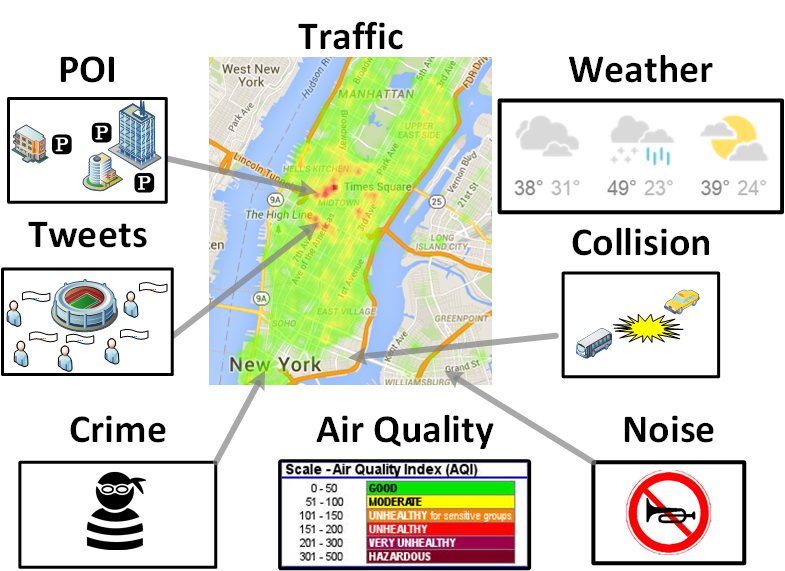
\includegraphics[width=0.9\textwidth]{fig/intro-data.png}
\caption{Use data collected in the urban space to address real urban problems.}
\label{fig:demo-data}
\end{figure}



\section{Take Crime Inference as an Example}

Understanding how to control crime is important because exposures to violence and crime have been unusually high in the U.S. for several decades and, while declining, they remain high~\cite{Baum05, Fink08}.Over half a million children and youth aged 10-24 years were treated in 2012 in emergency departments for nonfatal physical assault injuries related to gun shots, cuts and stabbings, among others~\cite{cdc15}.  Understanding the neighborhood context of crime is particularly important because victimization and other forms of crime exposures have many severe consequences.  Beyond the high medical bills and violent death, consequences include behavioral and mental health problems, aggression, substance abuse, post-traumatic stress disorder, and suicide, lower academic achievement, and engaging in further violence~\cite{Grai15}. 

In this paper, we study the problem of crime rate inference of communities. We select Chicago as the target of study for the following reason. Chicago has more homicides and non-negligent manslaughter rates (15.2)
per 100,000 residents than New York (4.0) and Los Angeles (6.5)
according to the FBI crime statistics for 2013 and has experienced no
decline in the past decade compared to the other two large cities,
which have been on a slow declining slope \cite{crime-stats}.


\begin{figure}[t]
\centering
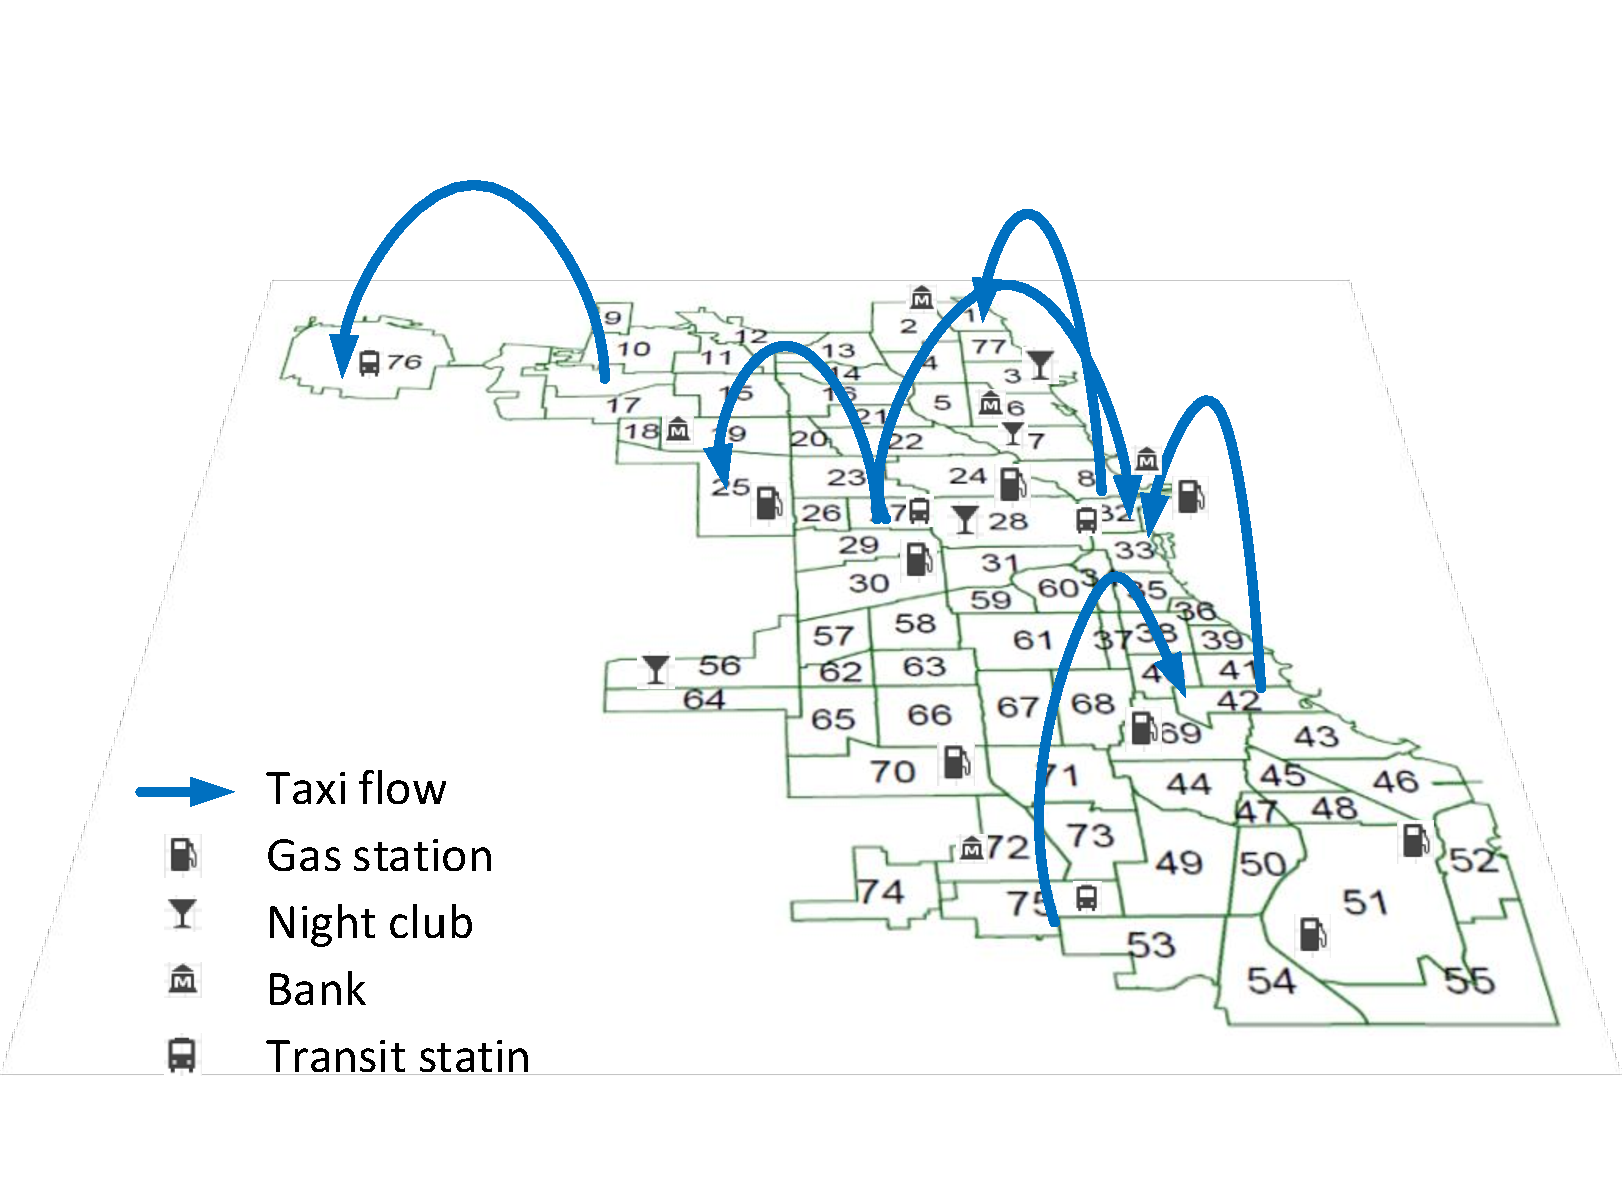
\includegraphics[width=0.8\textwidth]{fig/demo.pdf}
\caption{An illustration of various types of features we used in Chicago. The POI distribution across community areas reflects profiles of the region functionality. The taxi flow connects nonadjacent regions and act as a ``hyperlink''.}
\label{fig:demo}
\end{figure}

Traditionally, researchers have used demographic information (e.g., population poverty level, socioeconomic disadvantage, racial composition of population) to estimate the crime rate in a community~\cite{GrSa09}. However,  such demographic information only contains partial information about the neighborhoods and does not dynamically reflect the changes in the community (demographic survey is conducted by census bureau every 10 years). Using only demographic information will result in a relative error of at least 30\% for crime rate estimation in Chicago (refer to experiment section in the paper). Existing studies also use the geographical influence~\cite{Ans02} to estimate the crime rate, i.e., the crime in the nearby communities can be propagated to the focal community. But this geographical influence is of little help in improving the crime inference on top of demographic feature, with at most 0.4\% relative improvement in our experiments. This is probably because the nearby communities also share similar demographics, which limits the additional benefit of geographical influence.



Recently, big data reflecting city dynamics have become widely available~\cite{ZCWY14}, e.g., traffic flow, human mobility, social media, and crowd-generated Points-Of-Interest (POI). As shown in Figure~\ref{fig:demo}, such newer types of big data could provide us new insights to understand some traditional socioeconomic urban problems, such as crime rate inference problem we focus on in this paper. In particular, we propose to study two newer types of urban data: POI and taxi flow. 

\textbf{POI data.} POI data provide venue information such as GPS coordinates, category, popularity, and reviews. These POIs mostly belong to categories such as food, shop, transit, education, and etc. Recent studies have shown that using such categorical information of POIs are useful to profile neighborhood functions~\cite{YZX12}. And such neighborhood functions could further help us predict crime rate (e.g., communities with less education or entertainment facilities may have a higher rate of crime). Our experiments show that incorporating POI features   significantly improve the crime rate inference. Adding POI features in addition to demographics features reduces the relative error by at least 5\% in our experiments. This demonstrates that POI data provide additional information about the communities that is not covered by the demographics.

\textbf{Taxi flow data.} A huge amount of taxi flow data reflect how people commute in the city. In previous studies, when using geographical influence~\cite{Ans02}, people assume that a community is affected by the spatially nearby communities. However, communities are not only affected by spatially-close communities. Even if two communities are distant in geographical space, they could have a strong correlation if there are many people frequently travel between these two communities~\cite{GGM14}. We hypothesize that taxi flows may be considered as ``hyperlinks'' in the city that connect the locations and we use such data to estimate crime rates. Our experiments show very promising results --  adding taxi flow data on top of all other features can further decrease the error by 5\%.

We conduct extensive experiments including a systematic comparison between linear regression model and negative binomial model, tests of different combinations of  features, detailed discussions of how to construct features and why, analysis of features' relative importance, and theoretical interpretation of the results with a social scientist (a co-author in the paper). The experiments are conducted on the crime data over multiple years and using the modern big data show significant improvements.
